\documentclass[../Thesis.tex]{subfiles}
\begin{document}
\section{Đặt vấn đề}
% Tham khảo: https://machinelearningcoban.com/2017/07/09/prob/
Trong thời đại của công nghệ số, học tập trực tuyến đã trở thành một xu hướng phổ biến và ngày càng được nhiều người quan tâm đến. Đặc biệt, trong bối cảnh của đại dịch COVID-19,
E-learning đã trở thành một giải pháp thay thế cho hình thức học truyền thống khi nhiều quốc gia áp dụng chính sách phong tỏa và giãn cách xã hội.
E-learning là một hình thức giáo dục trực tuyến, trong đó việc học tập được thực hiện thông qua mạng internet hoặc các phương tiện truyền thông điện tử khác. Nó cho phép học viên tiếp cận các tài liệu học tập và tham gia vào các hoạt động giảng dạy mà không cần đến lớp học truyền thống. E-learning có thể áp dụng cho nhiều lĩnh vực khác nhau, từ giáo dục đại học, đào tạo doanh nghiệp cho đến các khóa học trực tuyến dành cho công chúng.
Với sự phát triển của công nghệ thông tin, e-learning đang trở thành một xu hướng phổ biến trên toàn thế giới. Nó đem lại nhiều lợi ích, bao gồm tiết kiệm chi phí cho học viên, đáp ứng nhu cầu học tập linh hoạt và giúp cải thiện chất lượng giảng dạy.
Đồng thời e-learning cung cấp cho học viên sự thuận tiện và linh hoạt trong việc truy cập các khóa học từ bất kỳ đâu và bất kỳ khi nào, đồng thời giúp cho các giáo viên và giảng viên dễ dàng tạo và quản lý các nội dung học tập.

Tuy nhiên, e-learning cũng đặt ra nhiều thách thức về kỹ thuật, tổ chức và chất lượng giảng dạy. Vì vậy, để có thể tận dụng tối đa lợi ích của E-learning và giải quyết các thách thức này,
việc nghiên cứu và phát triển các công nghệ và hệ thống quản lý học tập trực tuyến (\textbf{LMS}) là rất quan trọng.
Hệ thống quản lý học tập (LMS) đã trở thành một công cụ không thể thiếu trong các tổ chức giáo dục đại học, giúp quản lý, theo dõi và tối ưu hóa quá trình học tập trực tuyến. Tuy nhiên, các hệ thống LMS hiện có trên thị trường chưa đáp ứng được nhu cầu đa dạng và phức tạp của các tổ chức giáo dục đại học tại Việt Nam.
Mục tiêu của đề tài nhằm \textbf{phát triển một hệ thống LMS từ nền tảng Canvas LMS để hỗ trợ việc quản lý học tập trực tuyến phù hợp cho các tổ chức giáo dục đại học tại Việt Nam}.

Để phát triển e-learning, các tổ chức giáo dục cần phải giải quyết một số vấn đề quan trọng.
Trong nước, một trong những vấn đề quan trọng của e-learning là về hạ tầng kỹ thuật. Việc cải thiện hạ tầng mạng internet, đưa công nghệ vào giảng dạy và học tập sẽ giúp nâng cao chất lượng e-learning tại Việt Nam. Ngoài ra, các tổ chức giáo dục cần đầu tư vào nội dung học tập và đảm bảo chất lượng giảng dạy để thu hút người học tham gia học tập trực tuyến.
Ở nước ngoài, một trong những vấn đề quan trọng của e-learning là về sự đồng nhất của tiêu chuẩn và nội dung giảng dạy. Các quốc gia cần có tiêu chuẩn chung để đảm bảo chất lượng của các khóa học trực tuyến và đồng thời tạo thuận lợi cho việc hợp tác giữa các tổ chức giáo dục đến từ các quốc gia khác nhau. Ngoài ra, việc tạo ra nội dung học tập phù hợp với đối tượng học tập và đáp ứng nhu cầu thị trường cũng là một vấn đề quan trọng.

Để giải quyết các vấn đề này, các tổ chức giáo dục cần phải đầu tư vào nghiên cứu và phát triển công nghệ để nâng cao chất lượng e-learning. Đồng thời, cần có chính sách và hệ thống quản lý học tập trực tuyến hiệu quả để đảm bảo việc triển khai e-learning được thực hiện một cách bền vững và hiệu quả.

Vậy thì, hệ thống quản lý học tập là gì? \textbf{Hệ thống quản lý học tập} - \textbf{Learning Management System} là một phần mềm hoặc một nền tảng trực tuyến được sử dụng để quản lý, cung cấp và theo dõi các khóa học trực tuyến, nội dung giáo dục và hoạt động giảng dạy. Nó là một công cụ hỗ trợ cho việc giảng dạy và học tập trực tuyến, giúp các giảng viên, giáo viên hoặc tổ chức giáo dục có thể tạo và quản lý các khóa học trực tuyến, quản lý học viên và các tài nguyên học tập, tạo các bài kiểm tra và bài tập, cung cấp các tài liệu học tập và thống kê các hoạt động của học viên.
Một số tính năng chính của hệ thống LMS bao gồm:
\begin{itemize}
    \item Quản lý học viên và giảng viên
    \item Quản lý khóa học và nội dung học tập
    \item Tạo, cập nhật và quản lý các nội dung học tập
    \item Tạo các bài kiểm tra và bài tập
    \item Cung cấp công cụ trò chuyện trực tuyến, thảo luận và hỗ trợ trực tiếp cho học viên
    \item Thống kê và đánh giá hoạt động của học viên
\end{itemize}

Thị trường \textbf{LMS} đã có sự phát triển đáng kể trong những năm gần đây, với nhiều nền tảng khác nhau để hỗ trợ nhu cầu ngày
càng tăng về học tập trực tuyến. Trong bối cảnh giáo dục và đào tạo tiếp tục phát triển, việc sử dụng \textbf{LMS} để quản lý và cung cấp các khoá
học trực tuyến đã trở thành một xu hướng không thể thiếu. Nhắc đến các nền tảng \textbf{LMS} phổ biến hiện nay, chúng ta có thể kể đến các nền tảng như Moodle, Blackboard, Canvas, Edmodo, Schoology, Google Classroom, …

\begin{figure}[ht!]
\centering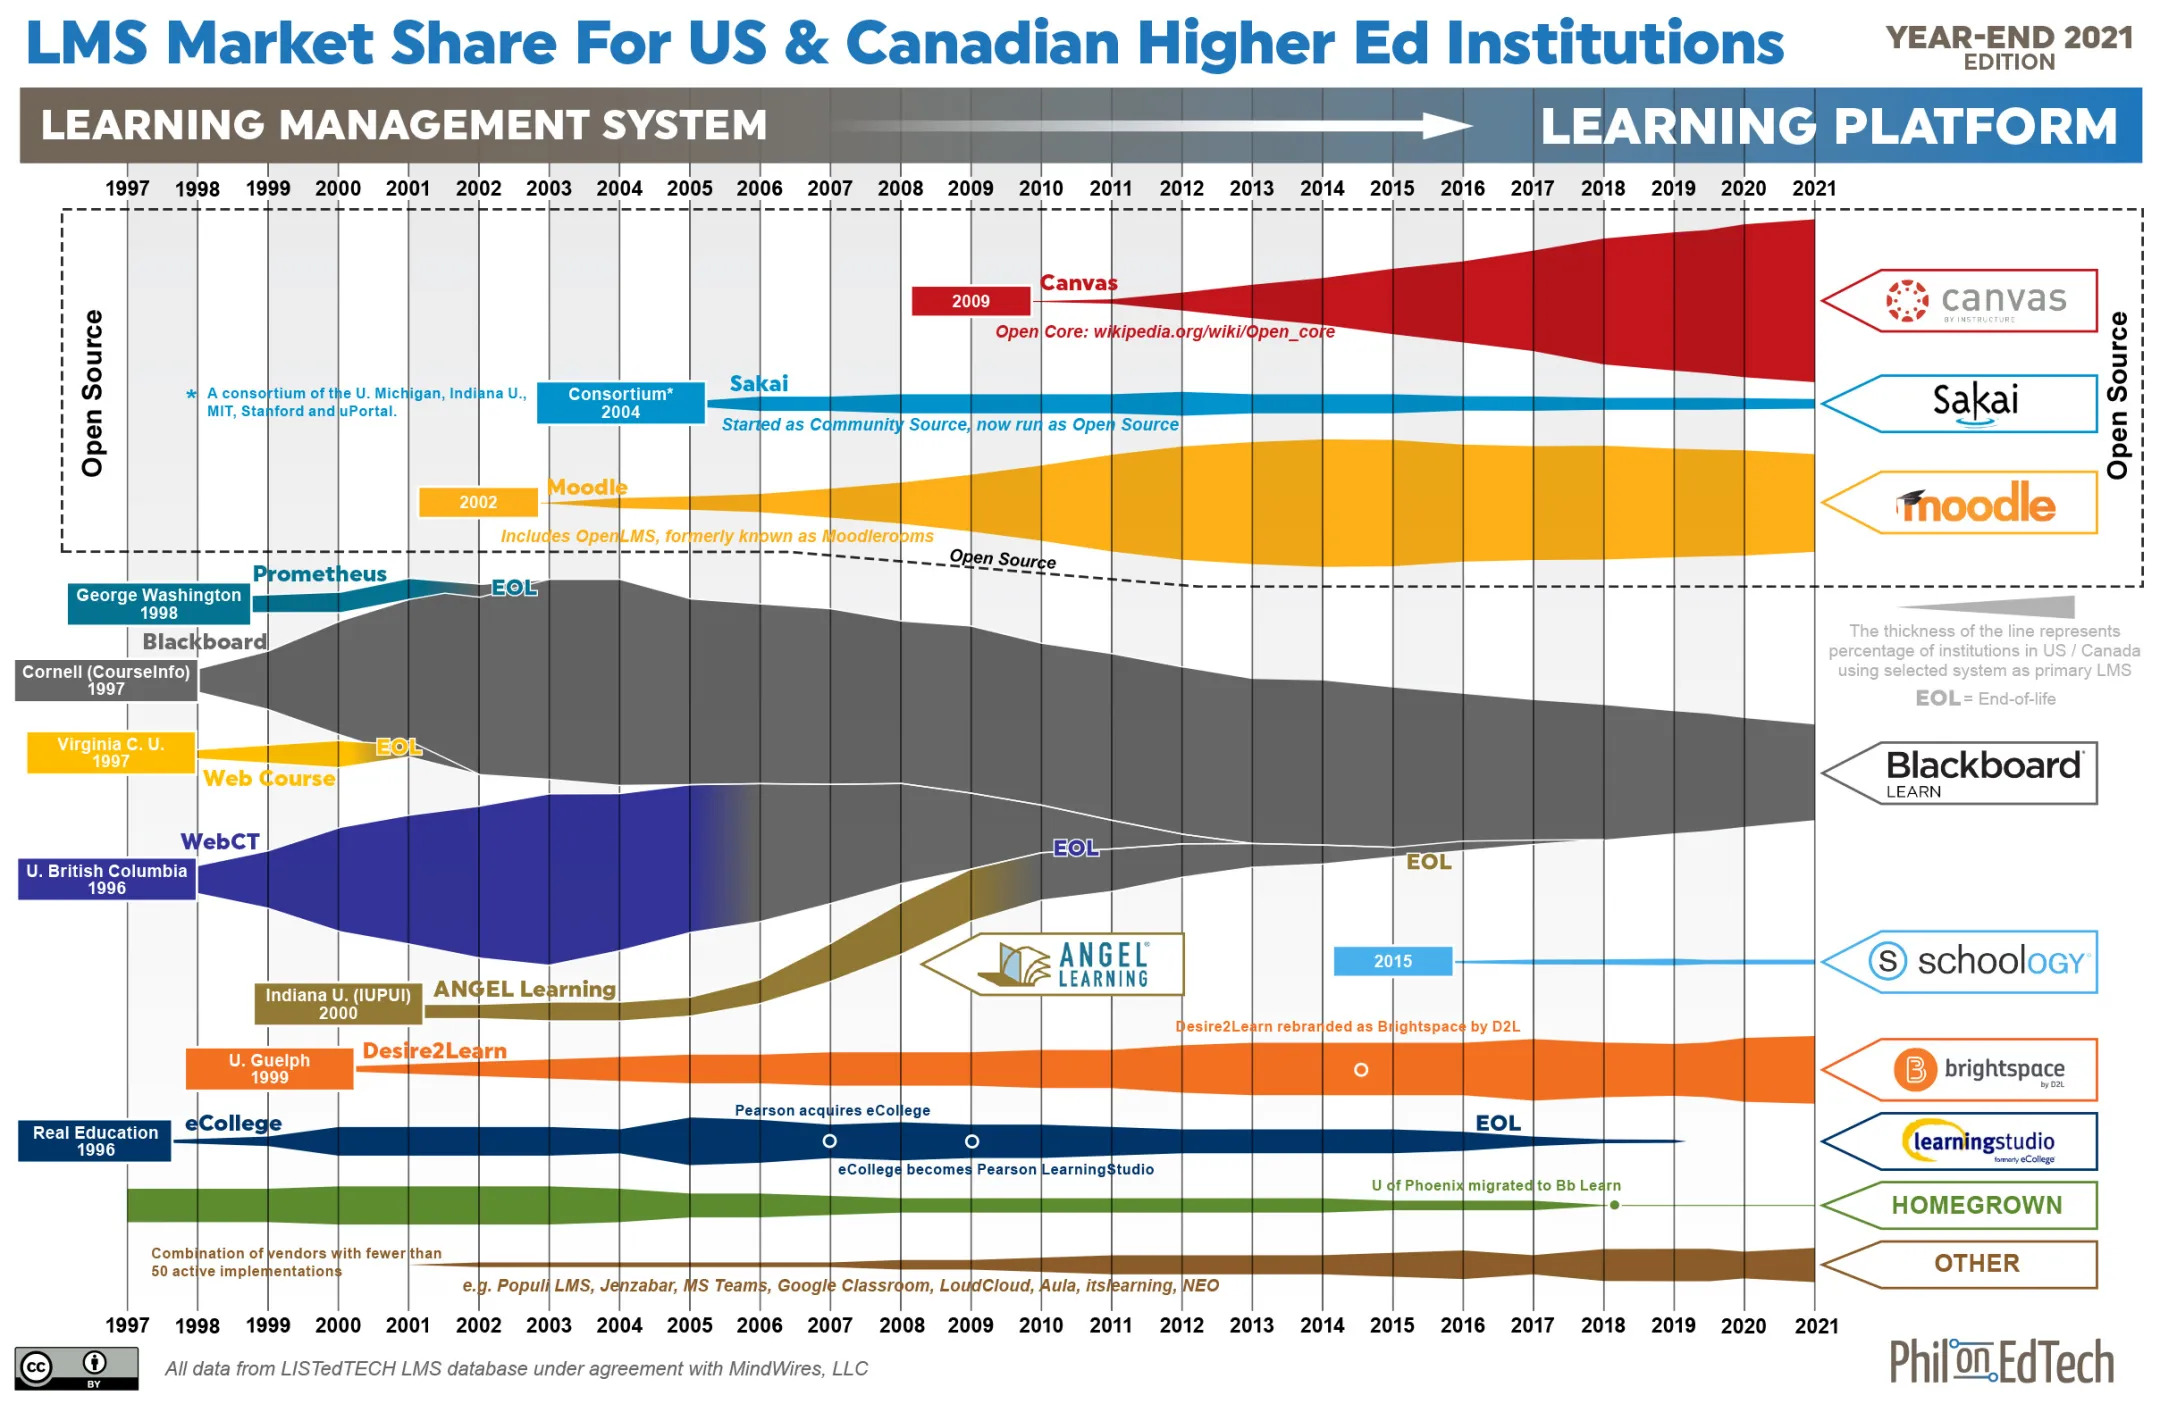
\includegraphics[scale=0.15]{lms-market}
\caption{Thị trường LMS tại Mỹ và Canada}
\label{fig:lms-market}
\end{figure}
% Tham khảo https://philhillaa.com/onedtech/state-of-higher-ed-lms-market-for-us-and-canada-year-end-2021-edition/

Thị phần của các hệ thống LMS phụ thuộc vào nhiều yếu tố như khu vực địa lý, loại tổ chức và mục đích sử dụng. Tuy nhiên, một số hệ thống LMS có thị phần lớn trên toàn thế giới bao gồm:

\begin{itemize}
    \item Moodle: Moodle là hệ thống LMS mã nguồn mở được sử dụng rộng rãi trên toàn thế giới, đặc biệt là trong giáo dục. Theo thống kê của Moodle, hệ thống LMS này được sử dụng trong hơn 200 quốc gia và có khoảng 200 triệu người dùng.
    \item Blackboard: Blackboard là hệ thống LMS thương mại phổ biến trong giáo dục và doanh nghiệp. Blackboard được sử dụng trong hơn 100 quốc gia và có khoảng 20 triệu người dùng.
    \item Canvas: Canvas là một hệ thống LMS được phát triển bởi công ty Instructure và được sử dụng rộng rãi trong giáo dục và doanh nghiệp. Theo thống kê của Instructure, Canvas có khoảng 30 triệu người dùng trên toàn thế giới.
    \item Google Classroom: Google Classroom là hệ thống LMS được cung cấp miễn phí bởi Google và được sử dụng phổ biến trong giáo dục. Tuy nhiên, không có con số chính thức về số lượng người dùng của Google Classroom.
\end{itemize}

Mỗi một hệ thống LMS đều có những ưu và nhược điểm riêng, tùy thuộc vào nhu cầu của từng tổ chức giáo dục.
Ví dụ, Moodle là một hệ thống LMS mã nguồn mở, miễn phí và có thể tùy chỉnh theo nhu cầu của tổ chức giáo dục. Tuy nhiên, Moodle có một số nhược điểm như thiếu tính linh hoạt trong việc tùy chỉnh giao diện, thiếu tính năng hỗ trợ trực tiếp cho học viên, thiếu tính năng đánh giá và thống kê hoạt động của học viên, …

Trong khi đó, Canvas là một hệ thống LMS thương mại, có tính linh hoạt cao trong việc tùy chỉnh giao diện, tính năng hỗ trợ trực tiếp cho học viên, tính năng đánh giá và thống kê hoạt động của học viên, … Tuy nhiên, Canvas có một số nhược điểm như giá thành cao, thiếu tính linh hoạt trong việc tùy chỉnh giao diện, thiếu tính năng hỗ trợ trực tiếp cho học viên, thiếu tính năng đánh giá và thống kê hoạt động của học viên, …
Nhưng đâu là lý do chính khiến Canvas LMS trở nên phổ biến trong thời gian gần đây.
\begin{itemize}
    \item Đầu tiên, Canvas LMS được thiết kế với giao diện người dùng thân thiện và dễ sử dụng, đồng thời cung cấp một loạt các tính năng và công cụ cho giảng viên và học sinh. Điều này giúp tăng tính hấp dẫn và sự tiện dụng của hệ thống.
    \item Canvas có thể tích hợp với nhiều công cụ và ứng dụng khác, bao gồm Google Drive, Microsoft Office, Turnitin và nhiều hơn nữa. Điều này giúp giảng viên và học sinh có thể sử dụng các công cụ khác nhau để tăng cường trải nghiệm học tập và quản lý thông tin.
    \item Canvas được xây dựng trên nền tảng đám mây, cho phép giảng viên và học sinh truy cập vào hệ thống từ bất kỳ địa điểm nào với kết nối Internet. Điều này giúp tăng tính ổn định và độ tin cậy của hệ thống.
    \item Canvas cung cấp hỗ trợ tuyệt vời cho giảng viên và học sinh thông qua các kênh như email, trò chuyện trực tiếp và điện thoại. Điều này giúp đảm bảo rằng người dùng có thể nhận được sự hỗ trợ cần thiết trong quá trình sử dụng hệ thống.
    \item Canvas được phát triển dựa trên mã nguồn mở, cho phép các nhà phát triển và tổ chức tùy chỉnh hệ thống để đáp ứng nhu cầu của họ. Điều này giúp tăng tính linh hoạt và tính mở rộng của hệ thống.
\end{itemize}

Nhưng không có hệ thống nào là hoàn hảo, Canvas cũng có một số nhược điểm đặc biệt là đối với các tổ chức giáo dục tại thị trường Việt Nam.

\begin{itemize}
    \item Đầu tiên, một trong những nhược điểm của Canvas LMS tại Việt Nam là vấn đề về tiếng Việt. Hệ thống này ban đầu được thiết kế và phát triển bằng tiếng Anh, do đó, việc sử dụng tiếng Việt trên Canvas LMS gặp nhiều khó khăn, đặc biệt là trong việc dịch thuật các tài liệu và hướng dẫn sử dụng cho người dùng Việt Nam. Điều này có thể gây khó khăn cho những người dùng không thành thạo tiếng Anh trong việc sử dụng hệ thống.
    \item Thứ hai, vấn đề về giá cả cũng là một nhược điểm của Canvas LMS tại Việt Nam. So với các hệ thống LMS khác trên thị trường Việt Nam, Canvas LMS có giá khá cao, đặc biệt là đối với các tổ chức giáo dục và doanh nghiệp nhỏ và vừa. Điều này có thể làm cho hệ thống này trở nên khó tiếp cận đối với một số khách hàng tiềm năng.
    \item Cuối cùng, một nhược điểm khác của Canvas LMS tại Việt Nam là việc phù hợp với một số nhu cầu đặc thù của khách hàng. Mặc dù Canvas LMS cung cấp nhiều tính năng và công cụ hữu ích cho quản lý học tập trực tuyến, tuy nhiên, nó không phải là giải pháp phù hợp cho tất cả các loại hình giáo dục và đào tạo. Ví dụ, nếu một tổ chức giáo dục có nhu cầu đặc biệt về tính năng hoặc quy trình riêng, thì họ có thể không tìm thấy giải pháp phù hợp trong Canvas LMS.
\end{itemize}

Vì vậy,  việc phát triển hệ thống quản lý học tập tùy chỉnh dựa trên Canvas LMS sẽ giúp các tổ chức giáo dục tại Việt Nam có thể tùy chỉnh hệ thống để phù hợp với nhu cầu học tập của sinh viên và cải thiện chất lượng giảng dạy trực tuyến là cần thiết. Hệ thống này cần được thiết kế với những tính năng và chức năng đáp ứng được nhu cầu đặc thù của các tổ chức giáo dục đại học tại Việt Nam. Một số tính năng và chức năng cần được đề xuất cho hệ thống quản lý học tập tùy chỉnh dựa trên Canvas LMS như sau:
\begin{itemize}
    \item Cập nhật giao diện bằng tiếng Việt
    \item Thiết kế giao diện đơn giản, dễ sử dụng, thân thiện với người dùng và tương thích với các thiết bị di động
    \item Tùy biến giao diện cho phù hợp với thị trường Việt Nam và thiết kế đẹp mắt
    \item Tích hợp với các công cụ phổ biến được sử dụng tại Việt Nam như Zalo, Viber, Facebook, GSuite, Microsoft Office,...
    \item Trên cơ sở của Canvas LMS, phát triển thêm các tính năng riêng biệt cho từng cơ sở giáo dục cụ thể.
\end{itemize}

Dựa trên nền tảng công nghệ của Canvas LMS và việc sử dụng các công nghệ mới như ReactJS, NodeJS, Ruby on rails ... để phát triển giao diện, hệ thống, hệ thống quản lý học tập tùy chỉnh dựa trên Canvas LMS sẽ giúp các tổ chức giáo dục tại Việt Nam có thể tùy chỉnh hệ thống để phù hợp với nhu cầu học tập của sinh viên và cải thiện chất lượng giảng dạy trực tuyến.

\section{Mục tiêu và phạm vi}

Mục tiêu của đồ án là xây dựng một hệ thống quản lý học tập linh hoạt và đáp ứng được nhu cầu đa dạng của các tổ chức giáo dục.

Cụ thể, đồ án nhằm tối ưu hóa các tính năng có sẵn trên nền tảng Canvas LMS, bao gồm quản lý khóa học, quản lý người dùng, quản lý tài liệu và bài tập, đánh giá và xếp loại, đồng thời tùy chỉnh để phù hợp với nhu cầu của các tổ chức giáo dục tại Việt Nam.

Phạm vi của đồ án sẽ tập trung vào việc phát triển các tính năng mới để tăng cường khả năng quản lý và theo dõi tiến độ học tập của sinh viên, giúp giảng viên dễ dàng tạo và quản lý các nội dung học tập, tương tác với sinh viên, đồng thời tạo điều kiện cho sinh viên tham gia và tương tác với nhau trong quá trình học tập. Ngoài ra, đồ án cũng sẽ tập trung vào việc tùy chỉnh giao diện để phù hợp với yêu cầu của từng tổ chức giáo dục cụ thể.
\section{Phương pháp}
Phương pháp nghiên cứu của đồ án sẽ bao gồm nhiều bước tiến hành khác nhau nhằm đảm bảo độ chính xác và tính khả thi của hệ thống.

Bước đầu tiên sẽ là khảo sát và phân tích nhu cầu của các tổ chức giáo dục đại học, tìm hiểu về các mô hình học tập trực tuyến đang được sử dụng và các yêu cầu cụ thể của học viên, giảng viên và quản lý. Sau đó, chúng ta sẽ tiến hành thiết kế hệ thống bao gồm các thành phần cơ bản như giao diện người dùng, tính năng quản lý học tập và đánh giá.

Sau khi hoàn thành thiết kế, chúng ta sẽ tiến hành phát triển và triển khai hệ thống, sử dụng các công nghệ hiện đại như HTML5, CSS3, JavaScript, ReactJS... Dựa trên nền tảng mã nguồn mở Canvas LMS để tạo ra một hệ thống LMS tùy chỉnh và đáp ứng được nhu cầu của các tổ chức giáo dục đại học.

Sau khi triển khai hệ thống, chúng ta sẽ tiến hành đánh giá và kiểm thử hệ thống để đảm bảo tính ổn định, độ tin cậy và hiệu quả của hệ thống. Cuối cùng, chúng ta sẽ tiến hành đào tạo cho nhân viên và người dùng về cách sử dụng và quản lý hệ thống để đảm bảo sự thích nghi và sử dụng hiệu quả của hệ thống trong các tổ chức giáo dục đại học.

\section{Kết quả dự kiến}

Đồ án có kết quả dự kiến đạt được là xây dựng một hệ thống quản lý học tập linh hoạt, dễ dàng tùy chỉnh và tích hợp nhiều tính năng hiện đại, giúp các tổ chức giáo dục đại học tại Việt Nam quản lý quá trình học tập, đào tạo, kiểm tra và đánh giá kết quả học tập của sinh viên một cách hiệu quả hơn. Bên cạnh đó, hệ thống còn hỗ trợ việc tương tác và trao đổi thông tin giữa sinh viên và giảng viên, giúp tạo ra một môi trường học tập trực tuyến chuyên nghiệp, tiện ích và tiết kiệm thời gian. Kết quả dự kiến của đồ án sẽ đóng góp vào việc nâng cao chất lượng giáo dục và đào tạo tại các tổ chức giáo dục đại học tại Việt Nam, đồng thời thúc đẩy sự phát triển của công nghệ và e-learning trong ngành giáo dục.
\end{document}
